% Gone, or Just Hidden? -- two-column paper version of REPORT.md.
% Build: tectonic main.tex   (or: pdflatex main && pdflatex main)   from the paper/ directory.
% Figures are read from ../docs/figures/ (written by scripts/18_scorecard.py and scripts/21_report_figures.py).
\documentclass[10pt,twocolumn,letterpaper]{article}

\usepackage{iftex}
\ifPDFTeX
  \usepackage[utf8]{inputenc}
  \usepackage[T1]{fontenc}
  \usepackage{newtxtext,newtxmath}
\else
  \usepackage{fontspec}
  \setmainfont{texgyretermes}[Extension=.otf, UprightFont=*-regular, BoldFont=*-bold, ItalicFont=*-italic,
    BoldItalicFont=*-bolditalic]
\fi
\usepackage[margin=0.75in,columnsep=0.25in]{geometry}
\usepackage{graphicx}
\usepackage{booktabs}
\usepackage{array}
\usepackage{amsmath}
\usepackage{xcolor}
\usepackage[font=small,labelfont=bf]{caption}
\usepackage{enumitem}
\usepackage[hidelinks]{hyperref}
\usepackage{url}

\graphicspath{{../docs/figures/}}
\setlist{nosep,leftmargin=*}
\newcommand{\eg}{e.g.\ }
\newcommand{\ie}{i.e.\ }

\title{\textbf{Gone, or Just Hidden? Auditing Unlearning of a Skill and a Book\\in the Hybrid LFM3-1.7B}}
\author{Anonymous Authors\\
\small AI Red Teaming, Safety \& Alignment Hackathon, Unlearning Track}
\date{November 2026}

\begin{document}
\maketitle

\begin{abstract}
Unlearning methods are usually judged on whether the model still answers direct prompts about the forgotten content.
We ask whether the content is gone or only hidden. We remove a body of memorised text (Harry Potter, following the
MUSE-Books protocol) and a skill (college calculus) from LiquidAI's LFM3-1.7B, a hybrid of gated short-convolution and
attention blocks. We run nine unlearning methods, including localized variants and weight edits written by AI agents,
and audit every model against prompt-side, training-free and fine-tuning attacks next to a reference that never
learned the content. Every method that passes the direct-prompt bar can be reversed. Calculus suppressed by RMU or by
an agent's rank-one patch returns with no training at all: projecting one direction out of each edited layer, using
the public base model as reference, restores 0.51 and 0.65 of a 0.71 target. No method erases calculus. The only result
close to erasure, held-out book passages at the never-trained floor under the strongest attack, comes from distilling
the model on data that lacks them, with or without an unlearning step. Collateral damage flows only to skills that
build on the forgotten one, and no component type of the hybrid holds the suppression. Finally, an editing agent that
tuned its edit against one relearning attack resisted that attack and nothing else, while tuning against sampled attack
configurations transferred to held-out attacks as a delay. Unlearning claims need a never-trained control,
training-free white-box attacks and relearning tested across configurations.
\end{abstract}

\section{Introduction}

Machine unlearning for large language models (LLMs) aims to remove hazardous knowledge, private data or copyrighted
content from a trained model while keeping its general capability \cite{shi2025muse,li2024wmdp}. Most evaluations ask
whether the model still produces the content when prompted, sometimes with paraphrases or jailbreaks. A growing body of
work shows that content that no longer appears in outputs can return after brief fine-tuning
\cite{hu2025jogging,lucki2024adversarial,doshi2024does}, and that defences claimed to be durable break under small changes
to the attack \cite{qi2025durability}.

We study this question on two targets of different kind, a body of memorised text and a skill learned in pretraining,
in a model family that unlearning studies have rarely examined. To our knowledge, LLM unlearning studies have almost
exclusively evaluated dense or mixture-of-experts transformers; the few that include hybrid models do not analyse the
non-attention blocks, and we know of no unlearning study on a gated short-convolution hybrid.

\paragraph{Contributions.}
\begin{itemize}
\item A full audit of nine unlearning methods on a book target and a calculus target in LFM3-1.7B, with prompt-side,
training-free and relearning attacks, a never-trained control, and bootstrap confidence intervals over test items.
\item A training-free attack that projects one direction per edited layer, estimated with the open base model, and
restores RMU-suppressed calculus without any gradient step.
\item Controls that separate unlearning from data effects: a matched distillation control shows that the most robust book
result (UNDO \cite{lee2025undo}) comes from the repair corpus, not from the unlearning step; cross-subskill relearning
(train on derivatives, score integrals) separates unmasking from re-teaching.
\item A depth ladder over arithmetic, algebra, precalculus and calculus showing that collateral damage flows only to
dependent skills.
\item Agent-written weight edits under a budget guard, including agents given a relearning probe, and the finding that
relearning resistance tuned on one attack configuration does not transfer while tuning on sampled configurations does.
\end{itemize}

\section{Related Work}

\paragraph{Hidden rather than removed.} Benign relearning on public, loosely related data restores knowledge from
unlearned LLMs \cite{hu2025jogging}. \L{}ucki et al.\ \cite{lucki2024adversarial} recover most of RMU's removed WMDP
knowledge with LoRA (rank 128) on 10 unrelated samples, and Doshi and Cooper Stickland \cite{doshi2024does} with generic
web text. Qi et al.\ \cite{qi2025durability} re-evaluate safeguards claimed to resist fine-tuning and break them with
small changes to the attack, such as the seed, the learning-rate schedule or the prompt template.

\paragraph{Robust unlearning.} NPO \cite{zhang2024npo} avoids the collapse of gradient ascent; RMU \cite{li2024wmdp}
perturbs internal representations on forget data; sharpness-aware minimisation improves resistance to relearning
\cite{fan2025sam}; invariance regularisation targets downstream fine-tuning \cite{wang2025ilu}; UNDO distils the
unlearned model into a noised copy \cite{lee2025undo}. Filtering the pretraining data builds safeguards that resist
tampering \cite{obrien2025deepignorance}, avoiding post-hoc removal altogether.

\paragraph{Directions and weight editing.} Single residual-stream directions mediate behaviours such as refusal and can be
ablated \cite{arditi2024refusal}. Recent work shows that LLMs can read and write neural-network weights directly
\cite{takehi2026sparks}; we let agents edit weights under an explicit budget. A fuller, source-checked survey is in the
project repository (\texttt{docs/RELATED\_WORK.md}).

\section{Setup}

\paragraph{Model.} LiquidAI/LFM3-1.7B has 24 layers: 13 gated short-convolution blocks, 5 sliding-window and 6 global
attention blocks. Every sublayer output passes through an RMSNorm (``sandwich'' norm) before it is added to the residual
stream; embeddings are tied. We use bf16, vLLM for evaluation and Hugging Face transformers for attacks that need hooks
or training.

\paragraph{Book target.} The base model barely knows the Harry Potter books (verbatim ROUGE-L F1 0.14). Following
MUSE \cite{shi2025muse}, we fine-tune a \emph{target} on the forget text plus two retain corpora and a \emph{retain-only}
model on the retain corpora alone, which serves as the never-trained floor. A KL anchor to the base model on FineWeb
keeps perplexity and MMLU at base level. Target versus retain-only: verbatim recall 0.944 vs 0.145 on 25 held-out test
passages; in-context knowledge-QA fact presence 0.22 vs 0.10.

\paragraph{Skill target.} College calculus (derivatives, indefinite and definite integrals, levels 1--3), generated and
graded with sympy; arithmetic, algebra and precalculus at the same levels form the retain sets. The target solves 0.80 of
150 test problems, reasoning in the visible answer. No model that never learned calculus exists; Section~\ref{sec:relearn}
uses cross-subskill relearning and training-free attacks instead.

\paragraph{Data and metrics.} Splits are 60/15/25 train/dev/test by source item (96k rows, deduplicated and
leakage-checked); all unlearning and selection decisions use train/dev only. Calculus accuracy is reported with
\emph{truncated} (hit the token cap), \emph{gibberish} and \emph{refused/abstained} rates, which never count as
forgetting; a run with $\ge$10\% gibberish or $>$45\% unfinished answers is \emph{degenerate}. Utility combines MMLU
(1{,}000 questions, 5-shot), IFEval (thinking mode), FineWeb perplexity and retain math into \texttt{utility\_rel}
relative to the target. The success bar, relative to the target, is: forget $\le$20\% on direct prompts, worst-case
recovery $\le$40\%, utility $\ge$95\%, perplexity $\le$1.1$\times$.

\section{Methods and Attacks}

\begin{table}[t]
\centering\small
\caption{Unlearning methods. 46 configurations were swept on dev; the best valid point per method and target was
audited on test.}
\label{tab:methods}
\begin{tabular}{@{}p{0.27\linewidth}p{0.66\linewidth}@{}}
\toprule
family & methods \\
\midrule
gradient & GA, GradDiff, GA with KL retain term \\
preference & NPO-KL (LoRA, all weights), SAM-NPO \cite{fan2025sam}; forget targets are the model's own solutions \\
representation & RMU \cite{li2024wmdp} (MLP down-projection of layers 2--4) \\
localized & attribution patching (0.5\% of parameters) + masked NPO / RMU; same-size random masks \\
distillation & UNDO \cite{lee2025undo}: shrink to 75\%, distil 105--157M tokens; controls distil the target itself \\
agent surgery & Claude agents edit weights under a guard (edit budget 0.1\% by low-rank count, 10--100 forward calls) \\
prompt & ``you have never read / do not know \ldots'' system prompt \\
\bottomrule
\end{tabular}
\end{table}

Table~\ref{tab:methods} lists the methods. Gradient methods collapsed the model at every learning rate tried; the
prompt baseline changed nothing. We audit each surviving model under three threat models.
\begin{itemize}
\item \textbf{Black box:} paraphrase, notation changes, word problems with a hidden calculus step, translation
(fr/de/es), jailbreak templates, best-of-16 with random augmentation, thinking mode, in-context examples, tool use
(sympy/calculator), re-derivation, and indirect and excerpt questions for the book. Attack sets were written by an LLM
and checked by deterministic verifiers.
\item \textbf{White box, no training:} abliteration \cite{arditi2024refusal}; direction projection at the edited
layers, with the direction estimated from forget-versus-contrast prompts or as the difference to the public base
model on forget prompts; INT8/INT4 quantization and weight noise; a Jacobian-lens readout.
\item \textbf{White box with data:} LoRA relearning on 20 forget-dev items (standard); all weights plus 200 chunks of
the unlearning text with test passages removed (book, three seeds); all weights or LoRA on 133 items, a 5$\times$
learning rate, learning-rate/schedule/seed grids; component-restricted LoRA; related data only (other math, generic web
text, up to 1{,}000 all-weight steps); cross-subskill relearning.
\end{itemize}

\section{Results}

\begin{figure*}[t]
\centering
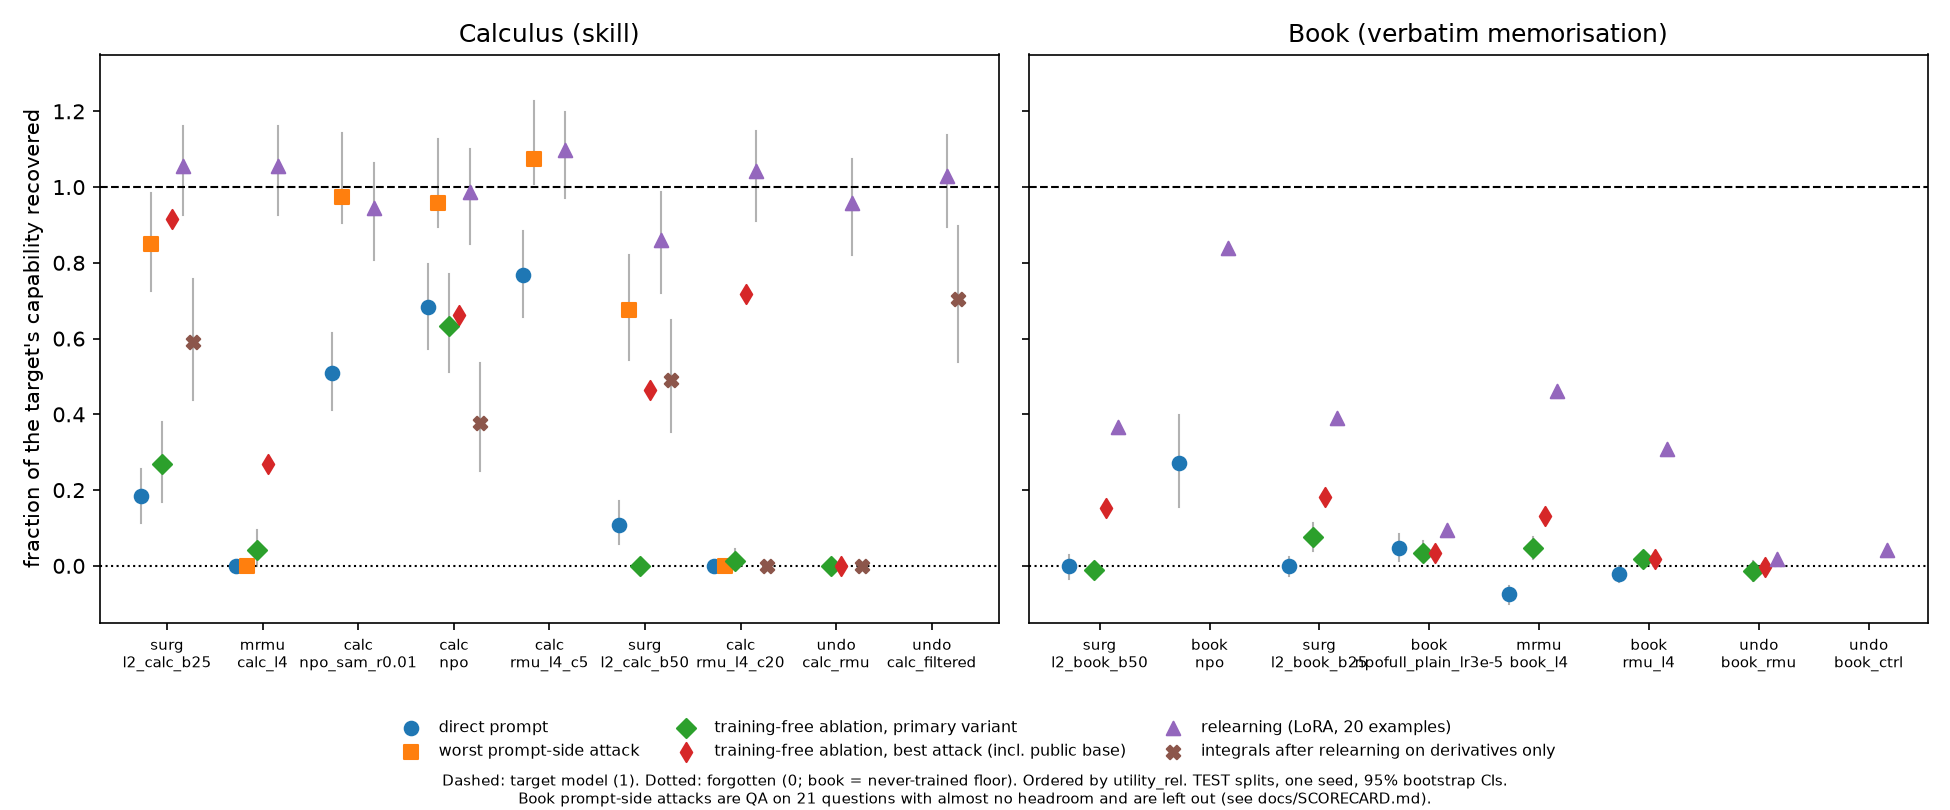
\includegraphics[width=\textwidth]{scorecard.png}
\caption{Fraction of the target's capability each attacker recovers, per method (test splits, 95\% bootstrap
intervals). A method that forgets should be near 0 in every column.}
\label{fig:scorecard}
\end{figure*}

\subsection{Direct forgetting and utility}

\begin{table}[t]
\centering\small
\caption{Direct forgetting on test (book: verbatim F1, floor 0.145, target 0.944; calculus: accuracy, target 0.80) and
\texttt{utility\_rel}. $^\ast$ = degenerate.}
\label{tab:direct}
\resizebox{\linewidth}{!}{%
\begin{tabular}{@{}lll@{}}
\toprule
model & direct forget & utility \\
\midrule
book RMU & 0.129 & 0.95 \\
book all-weight NPO-KL & 0.184 & 0.98 \\
book agent patch b25 / b50 & 0.144 / 0.144 & 0.99 / 0.99 \\
book UNDO (RMU teacher) & 0.127 & $\approx$0.89 (dev) \\
\midrule
calc NPO-KL (LoRA) & 0.547$^\ast$ (45\% truncated) & 0.99 \\
calc SAM-NPO & 0.407$^\ast$ (35\% truncated) & 0.99 \\
calc RMU c20 & 0.000$^\ast$ (91\% gibberish) & 0.98 \\
calc agent patch b25 & 0.147 (21\% truncated) & 0.995 \\
calc UNDO (RMU teacher) & 0.00$^\ast$ (93\% gibberish, dev) & $\approx$0.89 (dev) \\
\bottomrule
\end{tabular}}
\end{table}

Table~\ref{tab:direct} summarises direct forgetting. Book verbatim memorisation is removed to the never-trained floor
cheaply (RMU takes under a minute). Calculus has no clean trained method: below about half the target's accuracy,
every trained method degenerates. NPO stops finishing its answers; RMU jams the skill, producing gibberish on calculus
prompts only while retain math, MMLU, IFEval and perplexity stay at the target's level. The only non-degenerate calculus
result below 20\% is a rank-one patch written by an agent. Against the full bar, the book reaches it only with UNDO and
all-weight NPO (Section~\ref{sec:relearn}); no calculus model meets it.

\subsection{Prompt-side attacks}

No unlearned book model leaks: all stay at the floor within noise through all twelve black-box attacks. Book knowledge
QA has little headroom (target fact presence 0.19 vs 0.05 for the base model, $n=21$). Weak calculus unlearning leaks
through format: NPO and weak RMU recover 77--100\% of the target on at least one attack (notation 0.77; tool use 0.86,
equal to the target). SAM-NPO's extra forgetting is hidden: 0.41 directly but 0.78 with a tool. The RMU jam passes all
eleven calculus attacks at 0.00.

\subsection{Training-free attacks}

\begin{table*}[t]
\centering\small
\caption{Training-free recovery of calculus (accuracy on 100 test problems; target 0.71). The public-base projection
removes, at each edited layer, the direction from the open base model's mean activation on calculus prompts to the
unlearned model's. No gradient steps, no access to the unlearned-from model.}
\label{tab:trainfree}
\begin{tabular}{@{}lccccc@{}}
\toprule
model & edited weights & unablated & public-base & target, same & random \\
 & & & projection & projection & direction \\
\midrule
agent patch b25 (rank-one writes) & MLP out, layers 6--8 & 0.12 & \textbf{0.65} & 0.71 & 0.09 \\
RMU c20 & MLP out, layers 2--4 & 0.00 & \textbf{0.51} & 0.56 & 0.00 \\
masked RMU & units in layers 0--4 & 0.00 & 0.19 & -- & 0.00 \\
NPO / UNDO / removal patch b50 & -- / -- / layers 8--15 & 0.50 / 0.00 / 0.06 & 0.47 / 0.00 / 0.01 & 0.56 & -- \\
\bottomrule
\end{tabular}
\end{table*}

Table~\ref{tab:trainfree} shows the training-free attack. It restores the agent patch to 92\% and RMU to 72\% of the
target without training, with retain math unchanged; a random direction does nothing. A replication with new direction
prompts on 243 other test problems gives 0.43 (RMU) and 0.60 (patch) against 0.77--0.79 for the target. The patch's
edit is rank one, and the forget-versus-contrast estimate finds its write direction ($|\cos| = 0.997$ with the top
singular vector of the weight change). For RMU, that estimate removes the gibberish but not the forgetting, while the
base-model reference, available to anyone with the open weights, restores the skill. Under sandwich norms the site
matters: the MLP output before the norm works for the patch, the residual stream does not.

Quantization and weight noise recover nothing for any model. Abliteration at every layer removes calculus from the
target too, and on the book the projection removes the memorised text from the target, so both are uninformative there.
A Jacobian-lens readout misses the jam entirely: it finds intermediate calculus tokens in 0.15 of prompts on RMU
(control 0.14, other models 0.75--0.85), so an interpretability readout alone would call calculus erased.

\subsection{Relearning}\label{sec:relearn}

\begin{figure*}[t]
\centering
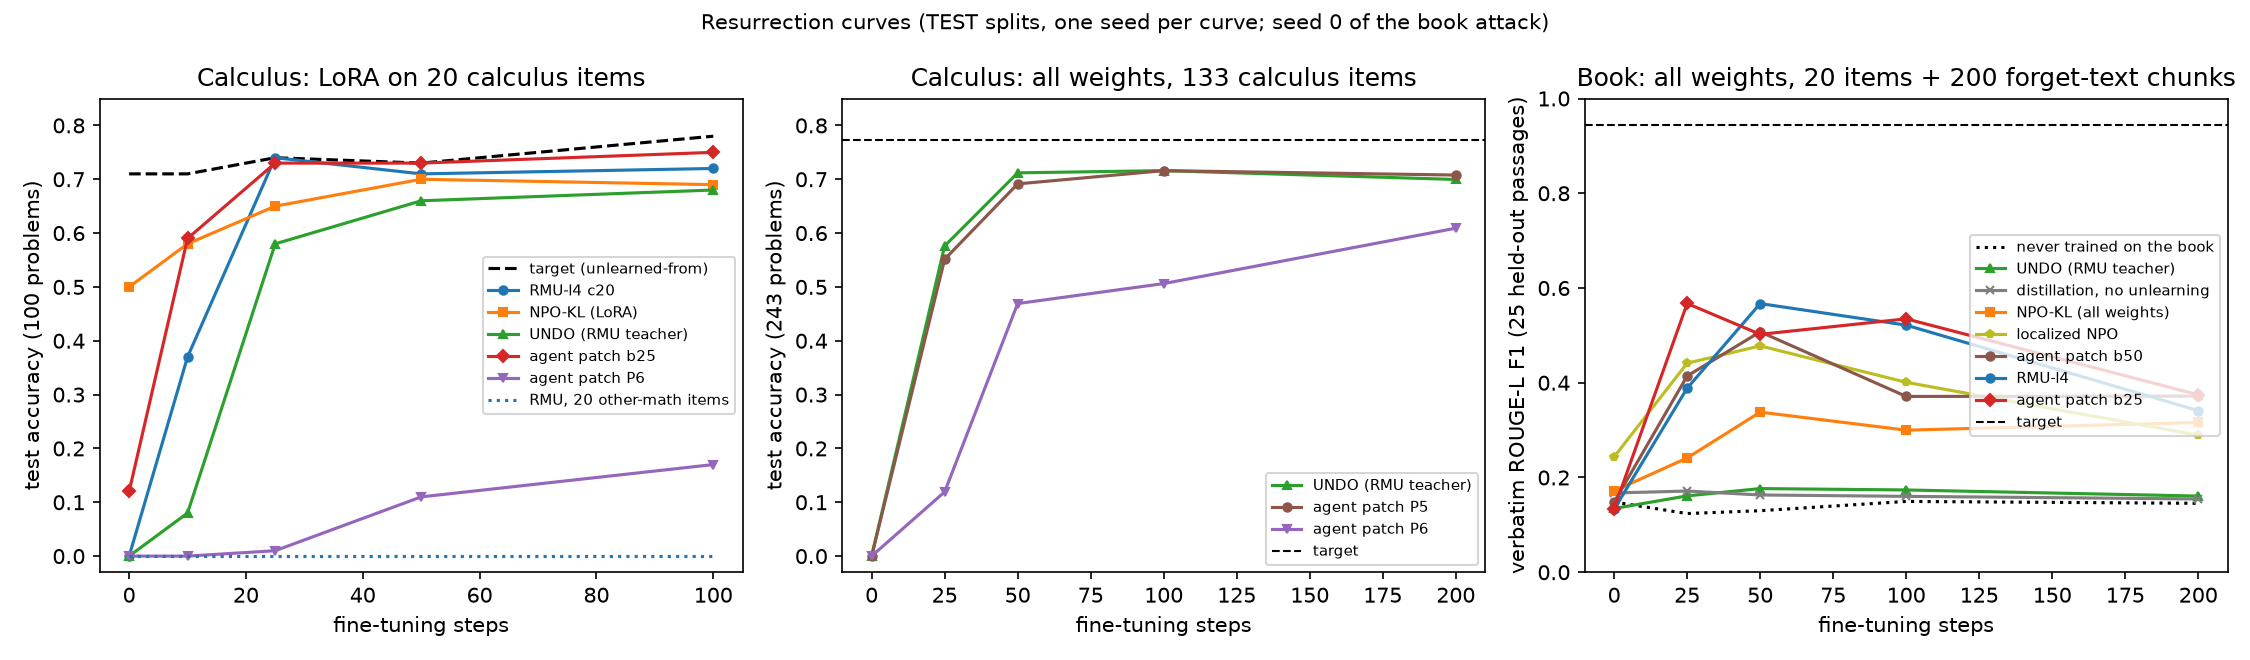
\includegraphics[width=\textwidth]{relearn_curves.png}
\caption{Resurrection curves on test. Left: LoRA on 20 calculus items. Middle: all-weight fine-tuning on 133 calculus
items. Right: book verbatim recall under all-weight fine-tuning with 200 chunks of the unlearning text (test passages
removed).}
\label{fig:relearn}
\end{figure*}

\paragraph{Standard attack.} LoRA on 20 forget-dev items restores calculus within 25 steps for RMU (0.74), the agent
patch (0.73) and NPO (0.65); UNDO follows more slowly (0.58 at 25, 0.68 at 100 steps; target 0.74--0.78). The same steps
on 20 other-math items leave every unlearned model where it started. On the book, RMU goes from 0.13 to 0.39 in 25
steps (31\% of the gap) while the never-trained control stays at 0.13--0.15, so the recovery comes from the unlearned
weights, not the fine-tuning data (Figure~\ref{fig:relearn}).

\begin{table}[t]
\centering\small
\caption{Strong book attack: share of the target's verbatim recall that returns (peak over 200 steps, mean and range
over three attack seeds).}
\label{tab:strong}
\begin{tabular}{@{}lr@{}}
\toprule
model & recovery \\
\midrule
never trained on the book & 0\% (0--1) \\
distillation from target, no unlearning & 3\% \\
UNDO, RMU teacher & 4\% (3--4) \\
all-weight NPO-KL & 25\% (24--25) \\
localized NPO & 42\% (42--43) \\
agent patch b50 & 43\% (39--45) \\
RMU & 50\% (45--53) \\
masked RMU, localized / random units & 54\% / 67\% \\
agent patch b25 & 59\% (53--65) \\
masked NPO, random units & 70\% (64--74) \\
\bottomrule
\end{tabular}
\end{table}

\paragraph{Strong book attack.} Table~\ref{tab:strong} orders the book methods. UNDO stays within about 0.03 of the floor
over a 16-configuration grid of learning rates, schedules and seeds, while all-weight NPO reaches 0.34--0.36; a higher
learning rate destroys memorisation in every model rather than restoring it.

\paragraph{Related data.} One thousand all-weight steps on 200 other-math solutions or on 1{,}000 FineWeb documents leave
RMU at 0.00--0.01, while web text leaves the target's calculus intact. This differs from published transformer results
\cite{lucki2024adversarial,doshi2024does}; the setups differ (skill versus hazardous facts, model, RMU layer and
coefficient, data), so we do not attribute the difference to the architecture. It is not evidence of erasure: the same
model returns with no training.

\begin{table}[t]
\centering\small
\caption{Cross-subskill relearning: integral accuracy (81 test problems) after LoRA on 20 derivative-only solutions, and
with 6 integral examples in the mix.}
\label{tab:xs}
\begin{tabular}{@{}lcc@{}}
\toprule
model & derivatives only (0 $\rightarrow$ 25 steps) & mixed \\
\midrule
target & 0.75 $\rightarrow$ 0.78 & -- \\
agent patch b25 & 0.04 $\rightarrow$ 0.44 & 0.62 \\
RMU c20 & 0.00 $\rightarrow$ 0.00 & 0.65 \\
UNDO & 0.00 $\rightarrow$ 0.00 & 0.52 \\
\bottomrule
\end{tabular}
\end{table}

\paragraph{Cross-subskill relearning.} A model without integration cannot learn it from derivative examples, and the
target gains nothing on integrals from these data (Table~\ref{tab:xs}). The patch regains integrals it never trained on
(two seeds; 69\% of the gain from mixed data), so its relearning partly unmasks. For RMU and UNDO, integrals stay at
0.00 (two seeds each, also under 200 all-weight steps) until integral examples are added. For RMU those integrals are
still present: the training-free attack restores them to 0.31 (target 0.56).

\paragraph{Component-restricted relearning.} Parameter-matched LoRA (2.3--2.8M parameters) on attention only, conv only or
MLP only restores RMU calculus to 0.70--0.75 by 100 steps, UNDO to 0.57--0.67 and the patch to 0.70--0.71. Conv-only
LoRA undoes a jam written into MLP weights; recovery speed follows the trainable-parameter count, not the component type.

\subsection{Erasure attempts}

\begin{figure*}[t]
\centering
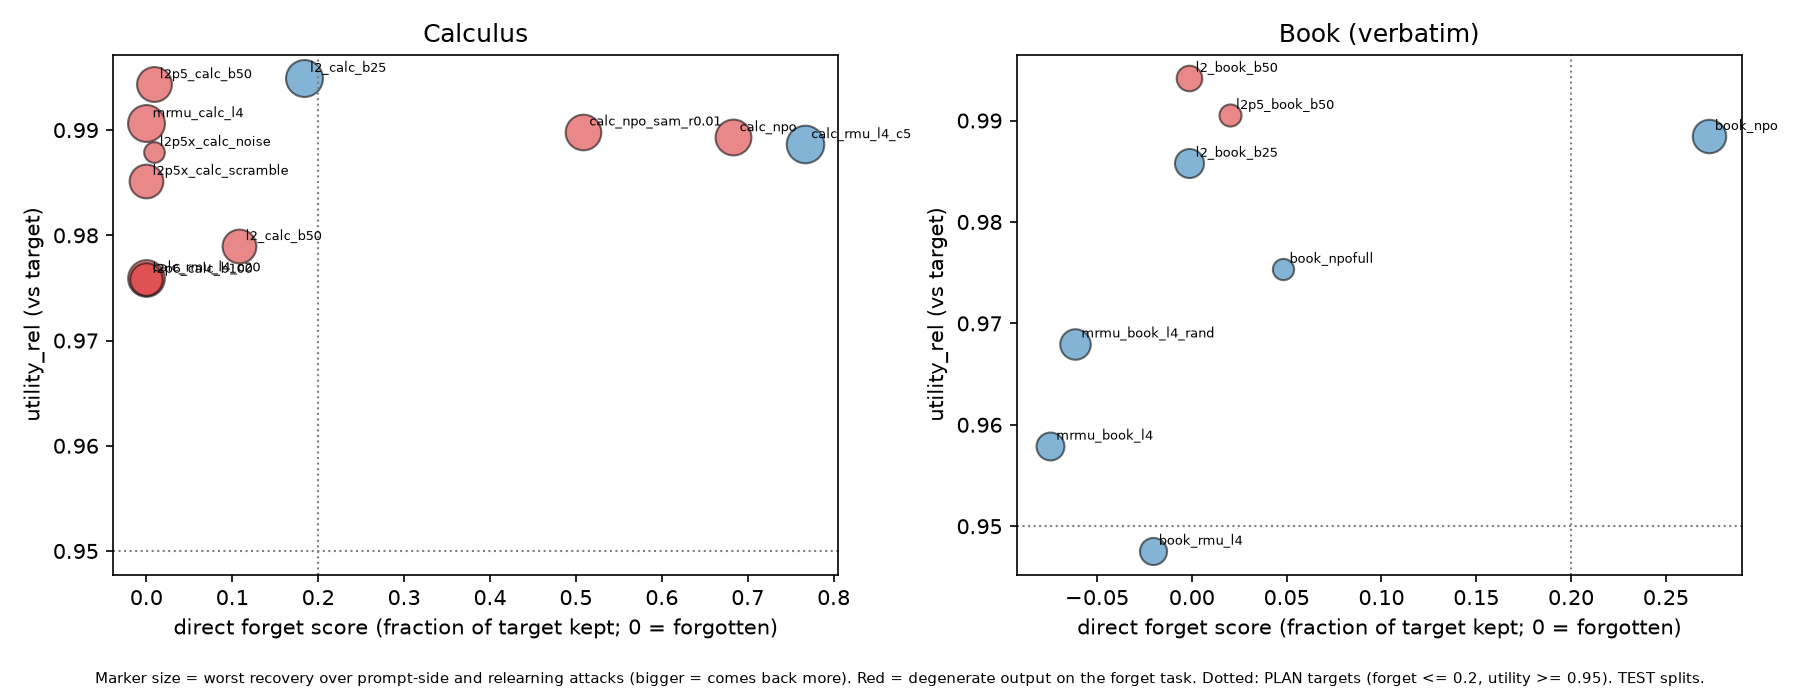
\includegraphics[width=0.92\textwidth]{tradeoff.png}
\caption{Direct forgetting versus utility; marker size is the worst recovery over prompt-side and relearning attacks,
red marks degenerate output on the forget task. Dotted lines: forget $\le$0.2 and utility $\ge$0.95.}
\label{fig:tradeoff}
\end{figure*}

\paragraph{Matched distillation control.} Distilling the plain target (no unlearning) with the UNDO recipe and book
mixture puts the held-out test passages at 0.168 (floor 0.145) with 3\% recovery under the strongest attack. Passages
present in the distillation corpus stay memorised (dev 0.64). Its utility cost matches UNDO's (MMLU 0.445, IFEval 0.61 on
dev). UNDO's book robustness therefore comes from what the repair corpus leaves out, not from the unlearning step.

\paragraph{Calculus-filtered distillation.} Removing calculus answers and 12{,}855 FineWeb documents with calculus
vocabulary from the repair data, with the target as teacher, reduces calculus from 0.71 to 0.39 without gibberish. Ten
LoRA steps on 20 calculus items restore 0.66, fifty restore the target level, and 20 other-math items alone reach 0.52.
Filtering the repair data erases recently fine-tuned text, not a pretrained skill (Figure~\ref{fig:tradeoff}). This
matches the literature, where the credible near-erasure results keep content out of the training data
\cite{obrien2025deepignorance}.

\subsection{Localization}

Calculus attribution is diffuse: forget and retain attribution have the same mix of component types and spread over
all 24 layers, and the selected 0.5\% of parameters holds 8.5\% of the attribution mass. Zeroing the selected units
collapses the model, localized masks forget no better than random masks of the same size, and masked RMU jams calculus
whichever units it may change. The book is more concentrated (16\% of the mass, mostly MLPs after global attention).
There, localized masks forget more than random ones and come back less under the strong attack (masked RMU 54\% vs 67\%;
masked NPO 42\% vs 70\%). Unit lists chosen by an agent did no better than random.

\subsection{Depth ladder}

\begin{figure}[t]
\centering
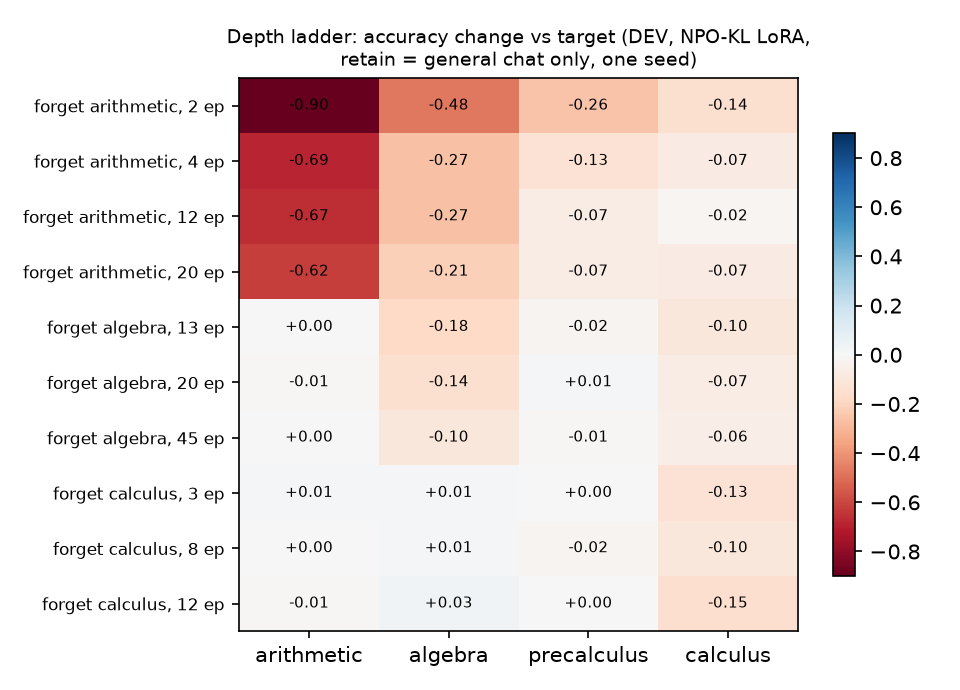
\includegraphics[width=\linewidth]{depth_ladder.png}
\caption{Accuracy change per topic when one topic is unlearned with NPO-KL (dev, one seed, 90 problems per topic).}
\label{fig:ladder}
\end{figure}

With general-chat retain data and dose set by the number of epochs (Figure~\ref{fig:ladder}), damage flows only upward.
Forgetting arithmetic (0.99 $\rightarrow$ 0.09--0.37) costs algebra 0.21--0.48, precalculus 0.07--0.26 and calculus
0.02--0.14. Forgetting algebra by 0.13--0.18 leaves arithmetic untouched and costs calculus 0.07--0.10. Forgetting
calculus costs nothing below it. When the other math topics are part of the retain set, NPO cannot remove arithmetic or
algebra at all. More epochs do not deepen NPO's forgetting, so arithmetic could not be matched to the other rungs.

\subsection{Agent weight surgery}

\begin{table*}[t]
\centering\small
\caption{Agent-written calculus patches (test). Relearning columns give accuracy after the attack (target 0.71 on 100
problems, 0.77 on 243). P5 and P6 had a relearning probe: P5 a single LoRA configuration, P6 sampled configurations.}
\label{tab:surgery}
\begin{tabular}{@{}llccc@{}}
\toprule
session & edit & direct & LoRA, 20 items, & all weights, 133 items, \\
 & & & 100 steps & 100 / 200 steps \\
\midrule
b25 (25 calls) & 3 rank-one MLP-out writes, layers 6--8 & 0.147 & 0.75 & -- \\
b50 (50 calls) & contrast-subspace removal, layers 8--15 & 0.087$^\ast$ & 0.60 & -- \\
P5 (50 calls) & rank-7 removal, all 24 layers & 0.007$^\ast$ & \textbf{0.29} & 0.72 / 0.71 \\
P6 (100 calls) & rank-7 negated write, all 24 layers & 0.000$^\ast$ & \textbf{0.17} & \textbf{0.51 / 0.61} \\
\bottomrule
\end{tabular}
\end{table*}

\begin{figure}[t]
\centering
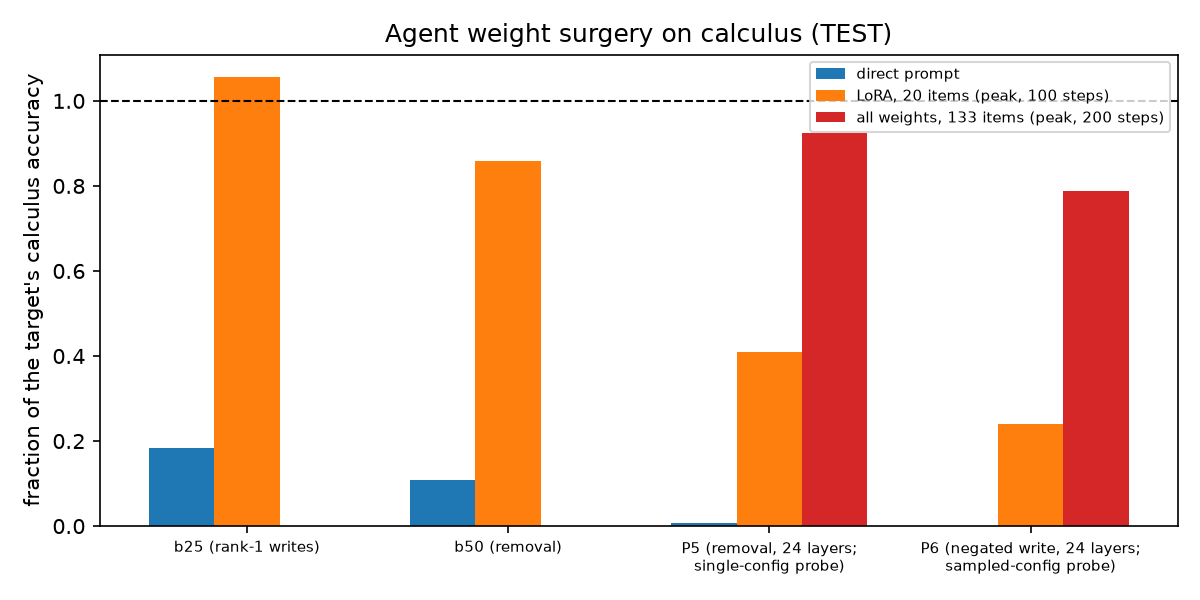
\includegraphics[width=\linewidth]{surgery.png}
\caption{Agent patches: direct forgetting and recovery under two relearning attacks, as fractions of the target.}
\label{fig:surgery}
\end{figure}

Claude agents edited weights through a harness that enforces an edit budget, a forward-call budget and a logged
rationale for every edit (Table~\ref{tab:surgery}, Figure~\ref{fig:surgery}). All patches fit the 0.1\% budget by
low-rank count (b25: 0.0017\%) but change 2.6--21\% of bf16 elements. The b25 patch behaves like trained RMU under every
attack and is undone training-free. Given a relearning probe with one configuration, the P5 agent found the most
relearning-resistant edit under that configuration, but with 133 items or a 5$\times$ learning rate it returns to
0.67--0.71 and 0.52. Tuning on sampled configurations (P6) held up better against every held-out family, and all
prompt-side and weight-level attacks give 0.00. It still returns to 79\% of the target after 200 all-weight steps, is
degenerate (89\% unfinished answers) and costs some retain math (0.933 vs 0.95) and book recall (0.833 vs 0.944). An
attacker with the public base model can copy the original weights back, so a sparse edit cannot be erasure against
that attacker by construction.

\section{Hypothesis Verdicts}

\begin{itemize}
\item \textbf{H1: unlearning suppresses rather than erases. Supported.} Every audited method is reversed by relearning,
the most suppressed calculus models also without training, and the never-trained control rules out learning from the
attack data. Two sub-claims fail: the Jacobian lens does not recover the forgotten calculus tokens, and RMU is not
uniformly more robust than NPO (worse than all-weight NPO on the book, and undone training-free on calculus where NPO is
not).
\item \textbf{H2: skills are harder to erase than facts. Supported, with a confound.} Calculus leaks through tool use and
notation where the book does not, and filtered distillation erases book text but only halves calculus. Book memorisation
was added by fine-tuning while calculus comes from pretraining.
\item \textbf{H3: collateral damage grows with how foundational the skill is. Supported in direction, partly in
magnitude.} Damage flows only to dependent skills; at matched forgetting this holds for algebra versus calculus.
\item \textbf{H4: localized edits forget as well with less collateral, random masks do not. Refuted for calculus, partly
supported for the book.}
\item \textbf{H5 (exploratory): forgotten content concentrates in particular components. Weak.} Calculus is diffuse; no
component type holds or undoes the suppression.
\item \textbf{H6 (exploratory): agentic surgery forgets measurably with $\le$0.1\% of weights.} Met under the low-rank
count, not by changed elements; always reversible, and every later calculus patch is degenerate.
\end{itemize}

\section{Discussion}

One direct-prompt score covered three different kinds of forgetting: a \emph{switch} that one projection per layer
turns off given the open base model (RMU, the rank-one patch); \emph{per-subskill suppression} that relearning lifts only
with examples of that subskill (RMU, UNDO); and \emph{no removable direction} but fast relearning (NPO, UNDO). The
evidence argues for evaluation practices that most unlearning studies omit:
\begin{itemize}
\item a never-trained control under the same attacks;
\item training-free white-box attacks that use the public base model;
\item relearning tested across configurations (data size, learning rate, all-weight versus LoRA, seeds), never only on
the configuration used for selection;
\item for skills, a cross-subskill test;
\item interpretability readouts treated as one-sided evidence: a lens that finds nothing has not found erasure.
\end{itemize}

\section{Limitations}

Each unlearning run uses one seed; book attacks use three attack seeds and most other numbers carry bootstrap intervals
over test items. Book sets are small (25 passages, 21 knowledge questions). No never-learned-calculus model exists. The
reference model loses about 24 points of thinking-off instruction following relative to base LFM3, as does the
retain-only model; all utility is relative to the reference. ``Best of $k$'' training-free variants were chosen on the
scored test problems; only the residual-stream variant was declared in advance. Agent surgery has one session per
design, selected on dev. Attack sets were written by an LLM with deterministic verifiers. All results concern one 1.7B
hybrid model.

\section*{Reproducibility and Use of AI}

Code, run specifications (one file per run naming the exact command), the frozen data manifest and a chronological log
of every run, decision and correction are in the project repository; data derived from MUSE and model checkpoints are
stored separately. Attack sets were written by Claude Sonnet 5.5 and checked by verifiers; weight edits were written by
Claude agents (Fable 5.2) under the budget guard; experiments were orchestrated with an AI coding agent.

\begin{thebibliography}{99}\small
\setlength{\itemsep}{2pt}

\bibitem{arditi2024refusal}
A.~Arditi, O.~Obeso, A.~Syed, D.~Paleka, N.~Panickssery, W.~Gurnee, N.~Nanda.
Refusal in language models is mediated by a single direction. \emph{NeurIPS}, 2024. arXiv:2406.11717.

\bibitem{doshi2024does}
J.~Doshi, A.~Cooper Stickland.
Does unlearning truly unlearn? A black box evaluation of LLM unlearning methods. arXiv:2411.12103, 2024.

\bibitem{fan2025sam}
C.~Fan, J.~Jia, Y.~Zhang, A.~Ramakrishna, M.~Hong, S.~Liu.
Towards LLM unlearning resilient to relearning attacks: A sharpness-aware minimization perspective and beyond.
\emph{ICML}, 2025. arXiv:2502.05374.

\bibitem{hu2025jogging}
S.~Hu, Y.~Fu, Z.~S.~Wu, V.~Smith.
Unlearning or obfuscating? Jogging the memory of unlearned LLMs via benign relearning. \emph{ICLR}, 2025.
arXiv:2406.13356.

\bibitem{lee2025undo}
B.~W.~Lee et al.
Distillation robustifies unlearning. \emph{NeurIPS}, 2025. arXiv:2506.06278.

\bibitem{li2024wmdp}
N.~Li et al.
The WMDP benchmark: Measuring and reducing malicious use with unlearning. \emph{ICML}, 2024. arXiv:2403.03218.

\bibitem{lucki2024adversarial}
J.~\L{}ucki, B.~Wei, Y.~Huang, P.~Henderson, F.~Tram\`er, J.~Rando.
An adversarial perspective on machine unlearning for AI safety. \emph{TMLR}. arXiv:2409.18025, 2024.

\bibitem{obrien2025deepignorance}
K.~O'Brien et al.
Deep ignorance: Filtering pretraining data builds tamper-resistant safeguards into open-weight LLMs.
arXiv:2508.06601, 2025.

\bibitem{qi2025durability}
X.~Qi et al.
On evaluating the durability of safeguards for open-weight LLMs. \emph{ICLR}, 2025. arXiv:2412.07097.

\bibitem{shi2025muse}
W.~Shi et al.
MUSE: Machine unlearning six-way evaluation for language models. \emph{ICLR}, 2025. arXiv:2407.06460.

\bibitem{takehi2026sparks}
Takehi, Teoh, Zhang, Khattab.
Sparks of weight-space programming: LLMs can natively read \& write neural network weights. Blog post, November 2026.

\bibitem{wang2025ilu}
C.~Wang et al.
Invariance makes LLM unlearning resilient even to unanticipated downstream fine-tuning. \emph{ICML}, 2025.
arXiv:2506.01339.

\bibitem{zhang2024npo}
R.~Zhang, L.~Lin, Y.~Bai, S.~Mei.
Negative preference optimization: From catastrophic collapse to effective unlearning. \emph{COLM}, 2024.
arXiv:2404.05868.

\end{thebibliography}

\end{document}
